\documentclass[11pt]{article}
% Shared preamble for the visualisation document.
\usepackage[margin=1.9cm]{geometry}
\usepackage{amsmath,amssymb,amsthm}
\usepackage{tikz}
\usepackage{tikz-cd}
\usetikzlibrary{arrows.meta,positioning,shapes.geometric,shapes.misc,calc,fit,
  backgrounds,decorations.pathmorphing,decorations.markings,patterns,matrix,
  chains,quotes,intersections}
\usepackage{booktabs}
\usepackage{rotating}
\setlength{\emergencystretch}{2.5em}
\usepackage{xcolor}
\usepackage[labelfont=bf,font=small]{caption}
\usepackage{newunicodechar}
% Lean source uses Unicode; map the characters that occur to TeX equivalents.
\newunicodechar{·}{\ensuremath{\cdot}}
\newunicodechar{α}{\ensuremath{\alpha}}
\newunicodechar{ᵒ}{\ensuremath{^{\mathrm{o}}}}
\newunicodechar{ᵈ}{\ensuremath{^{\mathrm{d}}}}
\newunicodechar{₀}{\ensuremath{_0}}
\newunicodechar{₁}{\ensuremath{_1}}
\newunicodechar{₂}{\ensuremath{_2}}
\newunicodechar{₃}{\ensuremath{_3}}
\newunicodechar{₄}{\ensuremath{_4}}
\newunicodechar{₅}{\ensuremath{_5}}
\newunicodechar{₆}{\ensuremath{_6}}
\newunicodechar{₇}{\ensuremath{_7}}
\newunicodechar{←}{\ensuremath{\leftarrow}}
\newunicodechar{→}{\ensuremath{\rightarrow}}
\newunicodechar{∘}{\ensuremath{\circ}}
\newunicodechar{≤}{\ensuremath{\le}}
\newunicodechar{⨆}{\ensuremath{\bigsqcup}}
\newunicodechar{⨅}{\ensuremath{\Inf}}
\usepackage{hyperref}
\hypersetup{colorlinks=true,linkcolor=blue!55!black,urlcolor=blue!55!black}

% ---- the four DAG tag colours -------------------------------------------
\definecolor{tagatomic}{RGB}{120,124,132}     % atomic
\definecolor{tagreducible}{RGB}{35,95,175}    % reducible
\definecolor{tagglue}{RGB}{25,130,85}         % glue
\definecolor{tagstructural}{RGB}{200,95,15}   % structural
\definecolor{bridgecol}{RGB}{155,45,150}      % bridges
\definecolor{diagcol}{RGB}{190,30,45}         % the diagonal
\definecolor{softgrey}{RGB}{238,238,240}

\newcommand{\Sup}{\bigsqcup}
\newcommand{\Inf}{\mathop{\rotatebox[origin=c]{180}{$\bigsqcup$}}}
\newcommand{\od}[1]{#1^{\mathrm{od}}}
\newcommand{\lean}[1]{\texttt{\small #1}}
% small typewriter label for use inside tikz-cd arrows
\newcommand{\lab}[1]{\text{\scriptsize\ttfamily #1}}
% shrink a commutative diagram to a given width (tikz-cd cannot be
% \resizebox'ed directly, so it is boxed first)
\newsavebox{\cdbox}
\newcommand{\cdwidth}{\textwidth}
\newenvironment{cdscale}[1]{\renewcommand{\cdwidth}{#1}\begin{lrbox}{\cdbox}}%
  {\end{lrbox}\resizebox{\cdwidth}{!}{\usebox{\cdbox}}}
\newcommand{\enn}{\mathbb{R}_{\ge 0}^{\infty}}

% ---- node styles ---------------------------------------------------------
\tikzset{
  latticept/.style={circle,draw=black!70,fill=white,inner sep=1.5pt,minimum size=5pt},
  cell/.style={draw=black!25,fill=softgrey,minimum size=1.05cm,inner sep=0pt,
               font=\footnotesize},
  diagcell/.style={cell,fill=diagcol!18,draw=diagcol!70,line width=.7pt,
               font=\footnotesize\bfseries},
  lem/.style={rounded corners=2pt,draw,fill=white,inner sep=3pt,
              font=\ttfamily\scriptsize,align=center,minimum height=6.5mm},
  atomic/.style={lem,draw=tagatomic,fill=tagatomic!10},
  reducible/.style={lem,draw=tagreducible,fill=tagreducible!10},
  glue/.style={lem,draw=tagglue,fill=tagglue!10},
  structural/.style={lem,draw=tagstructural,fill=tagstructural!12},
  use/.style={-{Stealth[length=2mm]},draw=black!55,line width=.5pt},
  bridge/.style={{Stealth[length=2mm]}-{Stealth[length=2mm]},draw=bridgecol,
                 dashed,line width=.8pt},
  dom/.style={-{Stealth[length=1.7mm]},draw=diagcol!85,line width=.5pt},
  ord/.style={draw=black!60,line width=.6pt},
  ghost/.style={draw=none,fill=none,inner sep=1pt},
}


\title{\bfseries Diagonal collapse for iterated suprema\\[2pt]
  \large a visual companion to the Lean development}
\author{}
\date{}

\begin{document}
\maketitle
\vspace{-2.2\baselineskip}

\begin{abstract}\noindent
This document draws the mathematics of the Lean files in \lean{RequestProject/}: the
theorem
\[
  \bigl(\forall i\,j,\ \exists k,\ F_{ij} \le F_{kk}\bigr)
  \ \Longrightarrow\
  \Sup_i \Sup_j F_{ij} \;=\; \Sup_k F_{kk},
\]
its two structural ingredients (currying and cofinality), the conditionally complete
variant and where its boundedness hypothesis is consumed, the dependency DAG of the
twenty-five lemmas as an actual graph, the seven bridges to other contexts as arrow
diagrams, and the catalogue of alternative proofs as a Boolean lattice of design
choices.  Every picture corresponds to a compiled Lean declaration; the caption names
it.
\end{abstract}

\tableofcontents
\medskip

\noindent\textbf{Where things live.}
\begin{center}\footnotesize
\begin{tabular}{@{}ll@{}}
\toprule
\lean{RequestProject/Diagonal.lean} & the core: currying, cofinality, boundedness \\
\lean{RequestProject/Applications.lean} & $\enn$, $\mathbb{N}_\infty$,
  \lean{Cardinal}, one topological corollary \\
\lean{RequestProject/Bridges.lean} & the same theorem in seven other contexts \\
\lean{RequestProject/ProofGraph.lean} & the dependency DAG, with \lean{decide}-checked
  invariants \\
\lean{RequestProject/Variations.lean} & ${\sim}40$ alternative proofs \\
\lean{RequestProject/MathlibPR.lean} & the upstreaming staging file \\
\bottomrule
\end{tabular}
\end{center}
\clearpage

\section{The statement, drawn}

Everything in \lean{RequestProject/Diagonal.lean} orbits one picture: a doubly indexed
family $F : \iota \to \iota \to \alpha$ is a \emph{square} of lattice elements, and the
hypothesis
\[
  h : \forall i\, j,\ \exists k,\ F_{ij} \le F_{kk}
\]
says that the \emph{diagonal} of that square is cofinal in it.  The conclusion
$\Sup_i \Sup_j F_{ij} = \Sup_k F_{kk}$ says the square and its diagonal have the same
supremum.

\begin{figure}[ht]
\centering
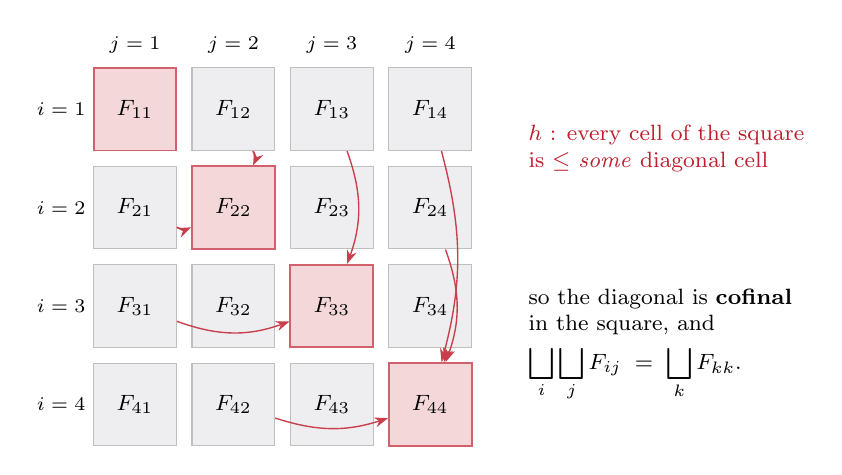
\begin{tikzpicture}[x=1.25cm,y=1.25cm]
  \foreach \i in {1,...,4}{
    \foreach \j in {1,...,4}{
      \ifnum\i=\j
        \node[diagcell] (c\i\j) at (\j,-\i) {$F_{\i\i}$};
      \else
        \node[cell] (c\i\j) at (\j,-\i) {$F_{\i\j}$};
      \fi
    }
  }
  % index labels
  \foreach \j in {1,...,4}{\node[font=\scriptsize] at (\j,-0.35) {$j=\j$};}
  \foreach \i in {1,...,4}{\node[font=\scriptsize] at (0.25,-\i) {$i=\i$};}
  % domination arrows: every cell is below some diagonal cell
  \draw[dom,bend left=25] (c12) to (c22);
  \draw[dom,bend left=20] (c13) to (c33);
  \draw[dom,bend left=15] (c14) to (c44);
  \draw[dom,bend right=25] (c21) to (c22);
  \draw[dom,bend left=20] (c24) to (c44);
  \draw[dom,bend right=20] (c31) to (c33);
  \draw[dom,bend right=18] (c42) to (c44);
  \draw[dom,bend left=18] (c34) to (c44);
  \node[font=\footnotesize,text=diagcol,align=left,anchor=west]
    at (4.9,-1.4) {$h$ : every cell of the square\\ is $\le$ \emph{some} diagonal cell};
  \node[font=\footnotesize,align=left,anchor=west]
    at (4.9,-3.4) {so the diagonal is \textbf{cofinal}\\ in the square, and\\[3pt]
      $\displaystyle\Sup_{i}\Sup_{j} F_{ij}\;=\;\Sup_{k} F_{kk}.$};
\end{tikzpicture}
\caption{The diagonal hypothesis of \lean{Golf.iSup2\_eq\_iSup\_diagonal} as a
combinatorial statement about a square: the red cells absorb everything.}
\end{figure}

\subsection{Three readings of the same supremum}

The proof of the collapse factors through a change of index: first the square is read as
one family over the product index (\lean{Golf.iSup\_pprod}, \emph{currying}), then the
diagonal is shown cofinal in it (\lean{Golf.iSup\_eq\_iSup\_of\_cofinal}).

\begin{figure}[ht]
\centering
\resizebox{\textwidth}{!}{%
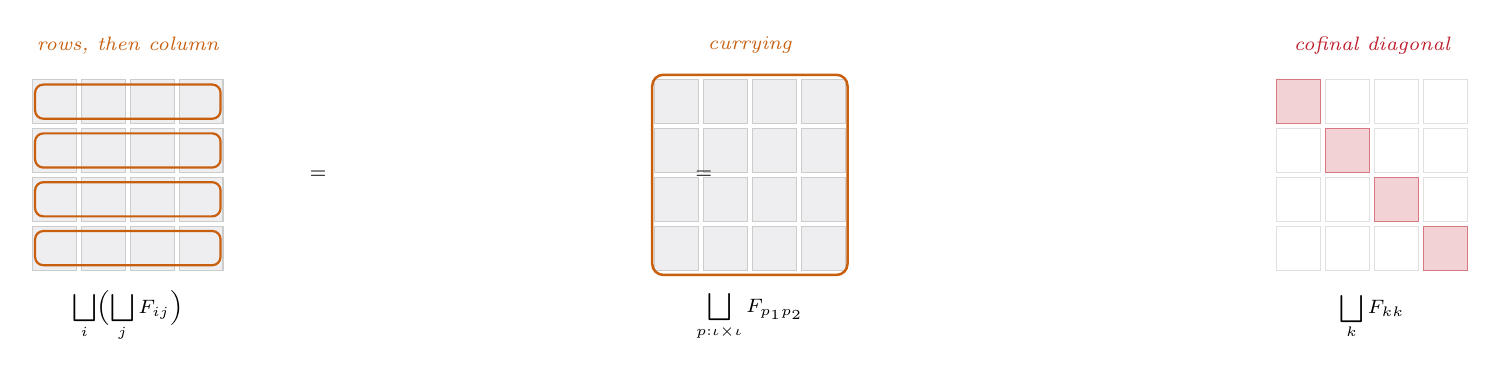
\begin{tikzpicture}[x=.62cm,y=.62cm,font=\scriptsize]
  % --- panel 1 : rows then columns
  \begin{scope}
    \foreach \i in {1,...,4}{\foreach \j in {1,...,4}{
      \fill[softgrey,draw=black!20] (\j-.45,-\i-.45) rectangle (\j+.45,-\i+.45);}}
    \foreach \i in {1,...,4}{
      \draw[rounded corners=3pt,tagstructural,line width=.8pt]
        (0.6,-\i-.35) rectangle (4.4,-\i+.35);}
    \node at (2.5,-5.4) {$\displaystyle\Sup_i\Bigl(\Sup_j F_{ij}\Bigr)$};
    \node[font=\scriptsize\itshape,text=tagstructural] at (2.5,0.15) {rows, then column};
  \end{scope}
  % --- equals
  \node at (6.4,-2.5) {$=$};
  % --- panel 2 : whole square at once
  \begin{scope}[xshift=7.9cm]
    \foreach \i in {1,...,4}{\foreach \j in {1,...,4}{
      \fill[softgrey,draw=black!20] (\j-.45,-\i-.45) rectangle (\j+.45,-\i+.45);}}
    \draw[rounded corners=4pt,tagstructural,line width=.9pt]
      (0.5,-4.55) rectangle (4.5,-0.45);
    \node at (2.5,-5.4) {$\displaystyle\Sup_{p : \iota\times\iota} F_{p_1 p_2}$};
    \node[font=\scriptsize\itshape,text=tagstructural] at (2.5,0.15) {currying};
  \end{scope}
  \node at (14.3,-2.5) {$=$};
  % --- panel 3 : diagonal only
  \begin{scope}[xshift=15.8cm]
    \foreach \i in {1,...,4}{\foreach \j in {1,...,4}{
      \ifnum\i=\j
        \fill[diagcol!20,draw=diagcol!60] (\j-.45,-\i-.45) rectangle (\j+.45,-\i+.45);
      \else
        \fill[white,draw=black!12] (\j-.45,-\i-.45) rectangle (\j+.45,-\i+.45);
      \fi}}
    \node at (2.5,-5.4) {$\displaystyle\Sup_k F_{kk}$};
    \node[font=\scriptsize\itshape,text=diagcol] at (2.5,0.15) {cofinal diagonal};
  \end{scope}
\end{tikzpicture}}
\caption{The two structural steps of the development.  The first equality is
\lean{iSup\_pprod} (true always); the second is \lean{iSup\_eq\_iSup\_of\_cofinal}
(true under $h$).}
\end{figure}

\subsection{The lattice picture of \texttt{le\_antisymm}}

Both structural lemmas are proved by antisymmetry: two families with a supremum each,
and two cofinality arrows.  As a Hasse diagram, the proof squeezes two elements
together.

\begin{figure}[ht]
\centering
\resizebox{\textwidth}{!}{%
\begin{tikzpicture}[x=1.5cm,y=1.25cm]
  \node[latticept,label=above:{$\Sup_i f_i$}] (sf) at (0,2) {};
  \node[latticept,label=above:{$\Sup_j g_j$}] (sg) at (3,2) {};
  \node[latticept,label=left:{$f_i$}] (fi) at (-0.6,0.6) {};
  \node[latticept,label=left:{$f_{i'}$}] (fi2) at (0.5,0.2) {};
  \node[latticept,label=right:{$g_j$}] (gj) at (3.6,0.6) {};
  \node[latticept,label=right:{$g_{j'}$}] (gj2) at (2.5,0.2) {};
  \node[latticept,label=below:{$\bot$}] (bot) at (1.5,-0.9) {};
  \draw[ord] (fi) -- (sf); \draw[ord] (fi2) -- (sf);
  \draw[ord] (gj) -- (sg); \draw[ord] (gj2) -- (sg);
  \draw[ord] (bot) -- (fi); \draw[ord] (bot) -- (fi2);
  \draw[ord] (bot) -- (gj); \draw[ord] (bot) -- (gj2);
  \draw[dom,bend left=18] (fi) to node[above,font=\scriptsize,pos=.5]{$h_1$} (gj);
  \draw[dom,bend left=18] (gj2) to node[below,font=\scriptsize,pos=.5]{$h_2$} (fi2);
  \draw[{Stealth[length=2mm]}-{Stealth[length=2mm]},bridgecol,line width=.9pt]
    (sf) to node[above,font=\scriptsize,text=bridgecol]{$=$} (sg);
  \node[align=left,font=\footnotesize,anchor=west] at (4.6,1.1)
    {\lean{iSup\_eq\_iSup\_of\_cofinal}\\[2pt]
     $\le$\;:\;\lean{iSup\_mono' h₁}\\
     $\ge$\;:\;\lean{iSup\_mono' h₂}\\[2pt]
     two arrows, no witnesses};
\end{tikzpicture}}
\caption{Mutual cofinality forces equality of suprema: each element of one family
has an upper bound in the other, so neither supremum can be the larger.}
\end{figure}

\subsection{A concrete instance: $\enn$ and the sum of two suprema}

The headline application $(\Sup_i f_i)+(\Sup_j g_j) = \Sup_k (f_k+g_k)$ is the square of
sums $F_{ij}=f_i+g_j$: monotone $f,g$ over a directed index make the diagonal cofinal.

\begin{figure}[ht]
\centering
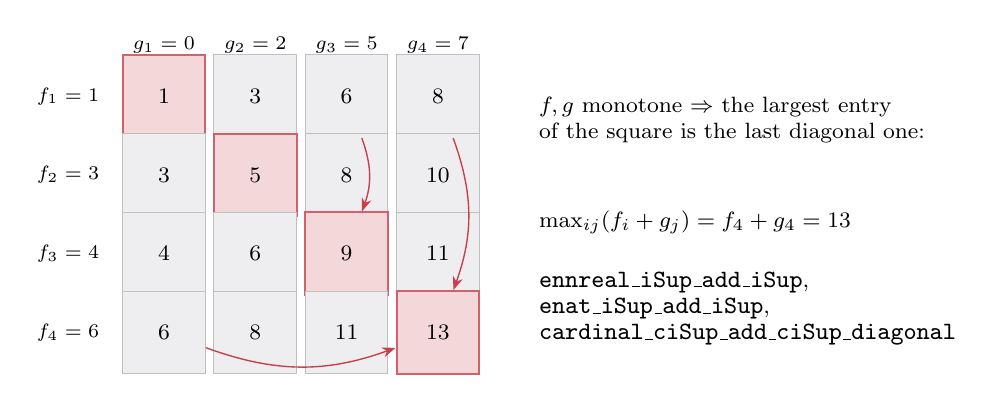
\begin{tikzpicture}[x=1.16cm,y=1.0cm,font=\scriptsize]
  \foreach \i/\fv in {1/1,2/3,3/4,4/6}{
    \foreach \j/\gv in {1/0,2/2,3/5,4/7}{
      \pgfmathtruncatemacro{\s}{\fv+\gv}
      \ifnum\i=\j
        \node[diagcell] (d\i\j) at (\j,-\i) {$\s$};
      \else
        \node[cell] (d\i\j) at (\j,-\i) {$\s$};
      \fi
    }
  }
  \foreach \j/\gv in {1/0,2/2,3/5,4/7}{\node at (\j,-0.35) {$g_\j=\gv$};}
  \foreach \i/\fv in {1/1,2/3,3/4,4/6}{\node at (-0.05,-\i) {$f_\i=\fv$};}
  \node[font=\footnotesize,align=left,anchor=west] at (5.0,-1.3)
    {$f,g$ monotone $\Rightarrow$ the largest entry\\
     of the square is the last diagonal one:};
  \node[font=\footnotesize,anchor=west] at (5.0,-2.6)
    {$\max_{ij} (f_i+g_j) = f_4+g_4 = 13$};
  \node[font=\footnotesize,align=left,anchor=west] at (5.0,-3.7)
    {\lean{ennreal\_iSup\_add\_iSup},\\ \lean{enat\_iSup\_add\_iSup},\\
     \lean{cardinal\_ciSup\_add\_ciSup\_diagonal}};
  \draw[dom,bend left=20] (d14) to (d44);
  \draw[dom,bend right=20] (d41) to (d44);
  \draw[dom,bend left=20] (d13) to (d33);
\end{tikzpicture}
\caption{A numerical square of sums.  Monotonicity of the two families is exactly what
makes the red diagonal absorb the square, which is why
\lean{ennreal\_iSup\_add\_iSup\_of\_monotone} needs no diagonal hypothesis.}
\end{figure}

\subsection{Where boundedness enters}

In a \emph{conditionally} complete lattice a supremum only behaves well below a ceiling.
The development is arranged so that the ceiling is used exactly once, in
\lean{Golf.ciSup\_pprod}; everything downstream inherits it.

\begin{figure}[ht]
\centering
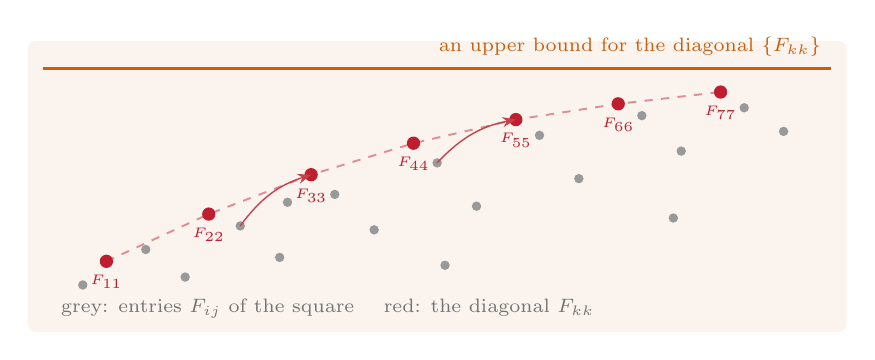
\begin{tikzpicture}[x=1.0cm,y=1.0cm,font=\footnotesize]
  \fill[tagstructural!7,rounded corners=3pt] (-0.3,-0.35) rectangle (10.1,3.35);
  \draw[line width=1pt,tagstructural] (-0.1,3.0) -- (9.9,3.0);
  \node[font=\scriptsize,text=tagstructural,anchor=south east] at (9.9,3.03)
    {an upper bound for the diagonal $\{F_{kk}\}$};
  % the diagonal: a rising red staircase, with its envelope
  \draw[diagcol!50,dashed,line width=.7pt]
    (0.7,0.55) -- (2.0,1.15) -- (3.3,1.65) -- (4.6,2.05) -- (5.9,2.35) --
    (7.2,2.55) -- (8.5,2.7);
  \foreach \k/\x/\y in {1/0.7/0.55,2/2.0/1.15,3/3.3/1.65,4/4.6/2.05,5/5.9/2.35,
                        6/7.2/2.55,7/8.5/2.7}{
    \fill[diagcol] (\x,\y) circle (2.4pt);
    \node[font=\tiny,text=diagcol,below=1.5pt] at (\x,\y) {$F_{\k\k}$};}
  % entries of the square: all under the envelope
  \foreach \x/\y in {0.4/0.25,1.2/0.7,1.7/0.35,2.4/1.0,2.9/0.6,3.6/1.4,4.1/0.95,
                     4.9/1.8,5.4/1.25,6.2/2.15,6.7/1.6,7.5/2.4,8.0/1.95,8.8/2.5,
                     9.3/2.2,5.0/0.5,3.0/1.3,7.9/1.1}{
    \fill[black!40] (\x,\y) circle (1.7pt);}
  \draw[dom,bend left=18] (4.9,1.8) to (5.9,2.35);
  \draw[dom,bend left=18] (2.4,1.0) to (3.3,1.65);
  \node[font=\scriptsize,text=black!55,anchor=west] at (0.0,-0.05)
    {grey: entries $F_{ij}$ of the square \quad red: the diagonal $F_{kk}$};
\end{tikzpicture}
\caption{Boundedness travels \emph{down} cofinality.  \lean{bddAbove\_range\_uncurry}
turns the diagonal hypothesis into \lean{isCofinalFor\_range\_iff} and then applies
\lean{IsCofinalFor.bddAbove}, transporting one ceiling from the diagonal to the whole
square.  That single transport is what feeds \lean{ciSup\_pprod}, \lean{bddAbove\_row}
and \lean{bddAbove\_range\_ciSup\_row}: the user of
\lean{ciSup₂\_eq\_ciSup\_diagonal} only ever has to bound the diagonal.}
\end{figure}

\subsection{Two concrete lattices}

The Boolean lattice $2^{\{a,b,c\}}$ makes the collapse tangible: take the two chains
$f = (\{a\},\{a,b\})$ and $g = (\{c\},\{b,c\})$.  Every join $f_i \sqcup g_j$ lies below
the last diagonal join $f_2 \sqcup g_2 = \{a,b,c\}$, so the double supremum collapses.

\begin{figure}[ht]
\centering
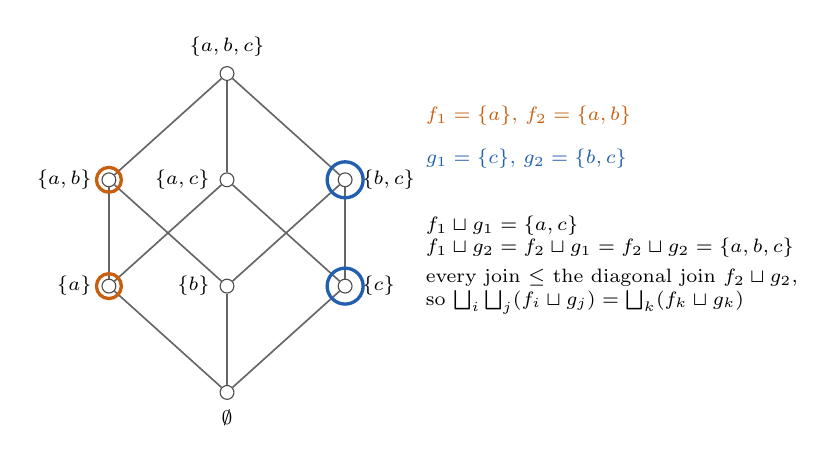
\begin{tikzpicture}[x=1.5cm,y=1.35cm,font=\scriptsize]
  \node[latticept,label=below:{$\emptyset$}]            (e)   at (0,0)  {};
  \node[latticept,label=left:{$\{a\}$}]                 (a)   at (-1,1) {};
  \node[latticept,label=left:{$\{b\}$}]                 (b)   at (0,1)  {};
  \node[latticept,label=right:{$\{c\}$}]                (c)   at (1,1)  {};
  \node[latticept,label=left:{$\{a,b\}$}]               (ab)  at (-1,2) {};
  \node[latticept,label=left:{$\{a,c\}$}]               (ac)  at (0,2)  {};
  \node[latticept,label=right:{$\{b,c\}$}]              (bc)  at (1,2)  {};
  \node[latticept,label=above:{$\{a,b,c\}$}]            (abc) at (0,3)  {};
  \foreach \x/\y in {e/a,e/b,e/c,a/ab,a/ac,b/ab,b/bc,c/ac,c/bc,ab/abc,ac/abc,bc/abc}
    {\draw[ord] (\x) -- (\y);}
  \foreach \n in {a,ab}{\draw[tagstructural,line width=1.2pt] (\n) circle (4.5pt);}
  \foreach \n in {c,bc}{\draw[tagreducible,line width=1.2pt] (\n) circle (6.5pt);}
  \node[font=\scriptsize,text=tagstructural,anchor=west] at (1.6,2.6)
    {$f_1=\{a\}$, $f_2=\{a,b\}$};
  \node[font=\scriptsize,text=tagreducible,anchor=west] at (1.6,2.2)
    {$g_1=\{c\}$, $g_2=\{b,c\}$};
  \node[font=\scriptsize,anchor=west,align=left] at (1.6,1.2)
    {$f_1\sqcup g_1=\{a,c\}$\\
     $f_1\sqcup g_2=f_2\sqcup g_1=f_2\sqcup g_2=\{a,b,c\}$\\[3pt]
     every join $\le$ the diagonal join $f_2\sqcup g_2$,\\
     so $\Sup_i\Sup_j (f_i\sqcup g_j)=\Sup_k (f_k\sqcup g_k)$};
\end{tikzpicture}
\caption{The diagonal hypothesis holds automatically here because both families are
monotone and the index order is directed --- the situation of
\lean{ennreal\_iSup\_add\_iSup\_of\_monotone} and
\lean{cardinal\_ciSup\_add\_ciSup\_of\_monotone}.}
\end{figure}

The hypothesis is not decoration.  In the three-element chain $0 < 1 < 2$, put
$F_{11}=F_{22}=0$ and $F_{12}=F_{21}=2$: no diagonal entry dominates $F_{12}$, and the
conclusion fails.

\begin{figure}[ht]
\centering
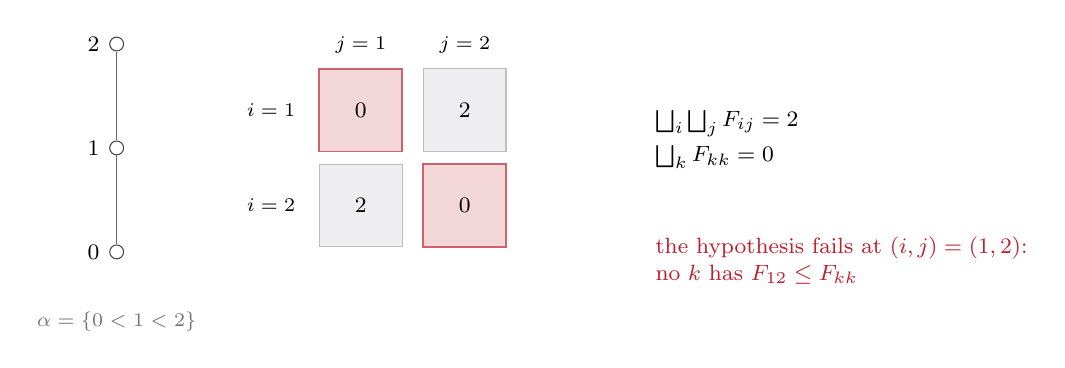
\begin{tikzpicture}[x=1.2cm,y=1.1cm,font=\footnotesize]
  % the chain
  \node[latticept,label=left:{$0$}] (z) at (0,0) {};
  \node[latticept,label=left:{$1$}] (o) at (0,1.2) {};
  \node[latticept,label=left:{$2$}] (t) at (0,2.4) {};
  \draw[ord] (z) -- (o) -- (t);
  \node[font=\scriptsize,text=black!55] at (0,-0.8) {$\alpha = \{0<1<2\}$};
  % the square
  \begin{scope}[xshift=3.1cm,yshift=1.8cm]
    \node[diagcell] (m11) at (0,0)     {$0$};
    \node[cell]     (m12) at (1.1,0)   {$2$};
    \node[cell]     (m21) at (0,-1.1)  {$2$};
    \node[diagcell] (m22) at (1.1,-1.1){$0$};
    \node[font=\scriptsize] at (0,0.75)   {$j=1$};
    \node[font=\scriptsize] at (1.1,0.75) {$j=2$};
    \node[font=\scriptsize] at (-0.95,0)   {$i=1$};
    \node[font=\scriptsize] at (-0.95,-1.1){$i=2$};
  \end{scope}
  \node[anchor=west,align=left] at (5.6,1.3)
    {$\Sup_i\Sup_j F_{ij} = 2$\\[2pt]
     $\Sup_k F_{kk} = 0$};
  \node[anchor=west,align=left,text=diagcol] at (5.6,-0.1)
    {the hypothesis fails at $(i,j)=(1,2)$:\\
     no $k$ has $F_{12} \le F_{kk}$};
\end{tikzpicture}
\caption{Why \lean{Golf.iSup₂\_eq\_iSup\_diagonal} needs its hypothesis.  Formally, the
$\ge$ direction is free (\lean{iSup\_mono'} with the witness $\langle k,k\rangle$); it is
the $\le$ direction that consumes $h$.}
\end{figure}

\subsection{The analytic corollary: a monotone staircase}

For monotone $f,g : \mathbb{N} \to \enn$ the diagonal family $k \mapsto f_k+g_k$ is
monotone too, so it converges to its supremum --- which, by the collapse, is
$(\Sup_i f_i)+(\Sup_j g_j)$.  That is \lean{Golf.ennreal\_tendsto\_add\_atTop}.

\begin{figure}[ht]
\centering
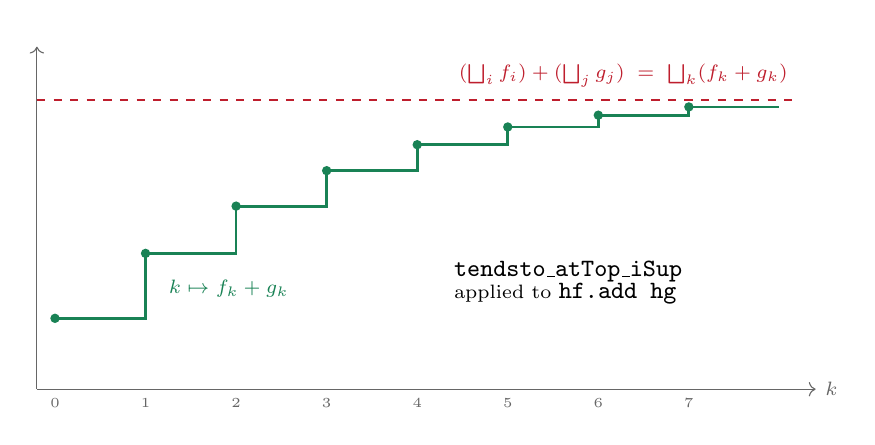
\begin{tikzpicture}[x=1.15cm,y=1.5cm,font=\scriptsize]
  \draw[->,black!60] (-0.2,0) -- (8.4,0) node[right] {$k$};
  \draw[->,black!60] (-0.2,0) -- (-0.2,2.9) node[above] {};
  \draw[diagcol,dashed,line width=.8pt] (-0.2,2.45) -- (8.2,2.45)
    node[right=-1pt,anchor=west,text=diagcol,xshift=2pt] {};
  \node[anchor=south east,text=diagcol,font=\scriptsize] at (8.2,2.47)
    {$(\Sup_i f_i)+(\Sup_j g_j) \;=\; \Sup_k (f_k+g_k)$};
  % staircase of f_k + g_k
  \draw[tagglue,line width=1pt]
    (0,0.6) -- (1,0.6) -- (1,1.15) -- (2,1.15) -- (2,1.55) -- (3,1.55) --
    (3,1.85) -- (4,1.85) -- (4,2.07) -- (5,2.07) -- (5,2.22) -- (6,2.22) --
    (6,2.32) -- (7,2.32) -- (7,2.39) -- (8,2.39);
  \foreach \x/\y in {0/0.6,1/1.15,2/1.55,3/1.85,4/2.07,5/2.22,6/2.32,7/2.39}{
    \fill[tagglue] (\x,\y) circle (1.7pt);}
  \foreach \x in {0,...,7}{\node[below,font=\tiny,text=black!60] at (\x,0) {\x};}
  \node[text=tagglue,anchor=west,font=\scriptsize] at (1.15,0.85) {$k \mapsto f_k+g_k$};
  \node[anchor=west,align=left,font=\scriptsize] at (4.3,0.9)
    {\lean{tendsto\_atTop\_iSup}\\ applied to \lean{hf.add hg}};
\end{tikzpicture}
\caption{The collapse is what identifies the limit of the diagonal sequence with the sum
of the two separate suprema; without it one only gets convergence to
$\Sup_k (f_k+g_k)$.}
\end{figure}

\clearpage

\section{The proof space as a graph}

\lean{RequestProject/ProofGraph.lean} reifies the spine of the development as a
\lean{SimpleGraph} on 25 nodes and proves its structural properties by \lean{decide}.
This section draws that graph.  Node colour is the tag, horizontal position is the rank
(= height in the DAG, \lean{Golf.Graph.rank}), and an arrow $b \to a$ means
``$a$ uses $b$'' (\lean{Golf.Graph.Uses}).

\begin{center}\footnotesize
\begin{tabular}{@{}llll@{}}
\toprule
\textcolor{tagatomic}{$\blacksquare$}~atomic & Mathlib, or one tactic & 10 nodes &
  \lean{card\_atomic}\\
\textcolor{tagreducible}{$\blacksquare$}~reducible & an iso/dual/rewrite collapses it &
  3 nodes & \\
\textcolor{tagglue}{$\blacksquare$}~glue & a small composition & 7 nodes & \\
\textcolor{tagstructural}{$\blacksquare$}~structural & introduces a new invariant &
  5 nodes & \lean{card\_structural}\\
\bottomrule
\end{tabular}
\end{center}

\begin{sidewaysfigure}
\centering
\resizebox{.96\textheight}{!}{%
\begin{tikzpicture}[x=1cm,y=1cm]
  % ---------------- rank 0 : atoms ----------------
  \node[atomic] (iSupMono)        at (0,10)   {iSup\_mono'};
  \node[atomic] (leAntisymm)      at (0,8.5)  {le\_antisymm};
  \node[atomic] (bddRow)          at (0,7)    {bddAbove\_range\_row};
  \node[atomic] (bddRowSups)      at (0,6)    {bddAbove\_range\_ciSup};
  \node[atomic] (cofinalRange)    at (0,4.5)  {isCofinalFor\_range\_iff};
  \node[atomic] (cofinalBdd)      at (0,3.5)  {IsCofinalFor.bddAbove};
  \node[atomic] (bddAdd)          at (0,2)    {bddAbove\_range\_add};
  \node[atomic] (csSupCofinal)    at (0,0.5)  {csSup\_eq\_csSup\_of\_\\forall\_exists\_le};
  \node[atomic] (colimitEqISup)   at (0,-1.2) {colimit\_eq\_iSup};
  \node[atomic] (finalDiag)       at (0,-2.4) {final\_diag\_of\_isFiltered};
  % ---------------- rank 1 ----------------
  \node[structural] (iSupPProd)   at (5,10)   {iSup\_pprod\\{\itshape currying}};
  \node[structural] (iSupCofinal) at (5,8.4)  {iSup\_eq\_iSup\_of\_cofinal\\{\itshape cofinality}};
  \node[structural] (ciSupPProd)  at (5,6.5)  {ciSup\_pprod\\{\itshape currying, bounded}};
  \node[glue] (ciSupCofinal)      at (5,5)    {ciSup\_eq\_ciSup\_of\_cofinal};
  \node[reducible] (bddUncurry)   at (5,3.9)  {bddAbove\_range\_uncurry};
  \node[structural] (ciSupLin)    at (5,0.5)  {ciSup\_eq\_ciSup\_of\_\\cofinal\_of\_linear};
  \node[structural] (finality)    at (5,-1.8) {iSup\_prod\_eq\_iSup\_\\diagonal\_functor};
  % ---------------- rank 2 ----------------
  \node[glue] (iSup2Cofinal)      at (10,9.2) {iSup₂\_eq\_iSup\_of\_cofinal};
  \node[glue] (ciSup2Diag)        at (10,5)   {ciSup₂\_eq\_ciSup\_diagonal};
  \node[glue] (bimonotone)        at (10,-1.8){iSup₂\_eq\_iSup\_diagonal\_\\of\_bimonotone};
  % ---------------- rank 3 ----------------
  \node[reducible] (iSup2Diag)    at (15,9.2) {iSup₂\_eq\_iSup\_diagonal};
  % ---------------- rank 4 ----------------
  \node[glue] (iSupOpDiag)        at (20,10.3){iSup\_op\_iSup\_diagonal};
  \node[reducible] (iInf2Diag)    at (20,8.1) {iInf₂\_eq\_iInf\_diagonal};
  % ---------------- rank 5 ----------------
  \node[glue] (ennrealAdd)        at (25,10.3){ennreal\_iSup\_add\_iSup};
  \node[glue] (cardinalAdd)       at (25,3.5) {cardinal\_ciSup\_add\_\\ciSup\_diagonal};
  % ---------------- rank guides ----------------
  \foreach \x/\r in {0/0,5/1,10/2,15/3,20/4,25/5}{
    \node[font=\small\itshape,text=black!45] at (\x,-3.6) {rank \r};}
  % ---------------- use edges (24) ----------------
  \draw[use] (leAntisymm) -- (iSupPProd);
  \draw[use] (leAntisymm) -- (iSupCofinal);
  \draw[use] (iSupMono)   -- (iSupCofinal);
  \draw[use] (leAntisymm) -- (ciSupPProd);
  \draw[use] (bddRow)     -- (ciSupPProd);
  \draw[use] (bddRowSups) -- (ciSupPProd);
  \draw[use] (leAntisymm) -- (ciSupCofinal);
  \draw[use] (csSupCofinal) -- (ciSupLin);
  \draw[use] (colimitEqISup) -- (finality);
  \draw[use] (finalDiag)  -- (finality);
  \draw[use] (cofinalRange) -- (bddUncurry);
  \draw[use] (cofinalBdd) -- (bddUncurry);
  \draw[use] (iSupPProd)  -- (iSup2Cofinal);
  \draw[use] (iSupCofinal)-- (iSup2Cofinal);
  \draw[use] (ciSupPProd) -- (ciSup2Diag);
  \draw[use] (ciSupCofinal) -- (ciSup2Diag);
  \draw[use] (bddUncurry) -- (ciSup2Diag);
  \draw[use] (finality)   -- (bimonotone);
  \draw[use] (iSup2Cofinal) -- (iSup2Diag);
  \draw[use] (iSup2Diag)  -- (iSupOpDiag);
  \draw[use] (iSup2Diag)  -- (iInf2Diag);
  \draw[use] (iSupOpDiag) -- (ennrealAdd);
  \draw[use] (ciSup2Diag) -- (cardinalAdd);
  \draw[use,rounded corners=6pt] (bddAdd) -- (2.2,2) -- (22.6,2) -- (cardinalAdd);
  % ---------------- bridge edges (2) ----------------
  \draw[bridge] (bimonotone) to[out=0,in=-80,looseness=.85]
    node[font=\small,text=bridgecol,pos=.45,sloped,above]{bridge} (iSup2Diag);
  \draw[bridge,rounded corners=8pt] (ciSupLin) -- (2.55,0.5) --
    node[font=\small,text=bridgecol,pos=.5,sloped,above]{bridge} (2.55,5) --
    (ciSupCofinal);
\end{tikzpicture}}
\caption{The dependency DAG of the development (\lean{Golf.Graph.G}), with the two
bridge links of \lean{Golf.Graph.G'} dashed in purple.  \lean{dep\_rank\_lt} states that
every solid arrow goes strictly left-to-right; \lean{atomic\_iff\_leaf} that the grey
nodes are exactly those with no incoming arrow; \lean{deps\_length\_le\_three} that no
node has more than three incoming arrows; \lean{card\_edges} that there are 24 solid
edges and \lean{card\_bridged\_edges} that the bridges cost exactly two more.}
\end{sidewaysfigure}

\subsection{Connectivity: a three-colouring, and the two bridges that kill it}

The interesting finding of \lean{ProofGraph.lean} is negative: the use-graph is
\emph{disconnected}.  The categorical route and the linear-order route reach the same
theorems through disjoint material.  This is proved by a graph colouring invariant
(\lean{colour\_eq\_of\_adj}, checked edge by edge with \lean{decide}, then propagated
along walks in \lean{colour\_eq\_of\_reachable}).

\begin{figure}[ht]
\centering
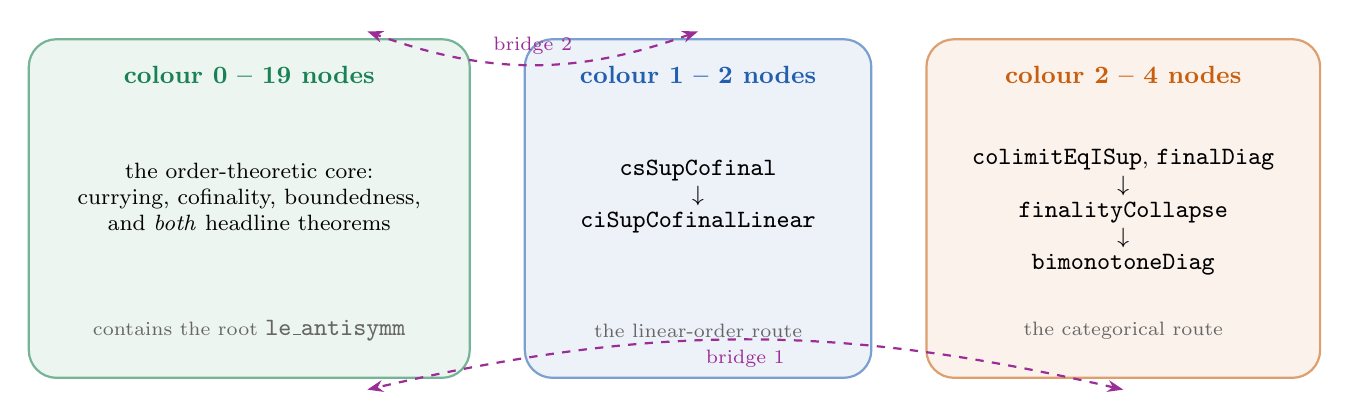
\begin{tikzpicture}[x=1cm,y=1cm,font=\footnotesize]
  \begin{scope}
    \draw[rounded corners=10pt,fill=tagglue!8,draw=tagglue!60,line width=.8pt]
      (0,0) rectangle (5.6,4.3);
    \node[font=\small\bfseries,text=tagglue] at (2.8,3.85) {colour 0 -- 19 nodes};
    \node[align=center] at (2.8,2.3)
      {the order-theoretic core:\\ currying, cofinality, boundedness,\\
       and \emph{both} headline theorems};
    \node[font=\scriptsize,text=black!60,align=center] at (2.8,0.6)
      {contains the root \lean{le\_antisymm}};
  \end{scope}
  \begin{scope}[xshift=6.3cm]
    \draw[rounded corners=10pt,fill=tagreducible!8,draw=tagreducible!60,line width=.8pt]
      (0,0) rectangle (4.4,4.3);
    \node[font=\small\bfseries,text=tagreducible] at (2.2,3.85) {colour 1 -- 2 nodes};
    \node[align=center] at (2.2,2.3)
      {\lean{csSupCofinal}\\ $\downarrow$\\ \lean{ciSupCofinalLinear}};
    \node[font=\scriptsize,text=black!60] at (2.2,0.6) {the linear-order route};
  \end{scope}
  \begin{scope}[xshift=11.4cm]
    \draw[rounded corners=10pt,fill=tagstructural!8,draw=tagstructural!60,line width=.8pt]
      (0,0) rectangle (5.0,4.3);
    \node[font=\small\bfseries,text=tagstructural] at (2.5,3.85) {colour 2 -- 4 nodes};
    \node[align=center] at (2.5,2.1)
      {\lean{colimitEqISup}, \lean{finalDiag}\\ $\downarrow$\\
       \lean{finalityCollapse}\\ $\downarrow$\\ \lean{bimonotoneDiag}};
    \node[font=\scriptsize,text=black!60] at (2.5,0.6) {the categorical route};
  \end{scope}
  \draw[bridge,bend left=20] (8.5,4.4) to
    node[above,font=\scriptsize,text=bridgecol]{bridge 2} (4.3,4.4);
  \draw[bridge,bend right=13] (13.9,-0.15) to
    node[below,font=\scriptsize,text=bridgecol]{bridge 1} (4.3,-0.15);
\end{tikzpicture}
\caption{\lean{not\_connected}: the colouring is constant on connected components and
takes three values, so \lean{G} is disconnected --- the categorical proof of the collapse
shares \emph{no} lemma with the order-theoretic one.  Adding the two purple bridge
edges makes the space connected (\lean{bridged\_connected}).}
\end{figure}

\subsection{Why connectivity is proved by descent, not by search}

Reachability is expensive for the kernel, so the positive statement is reduced to a
local one: a parent function \lean{toRoot} together with a strictly decreasing
\lean{depth}.  This is a spanning tree of the bridged graph, rooted at
\lean{le\_antisymm}.

\begin{sidewaysfigure}
\centering
\resizebox{.96\textheight}{!}{%
\begin{tikzpicture}[x=1cm,y=1cm,font=\scriptsize]
  \tikzset{tn/.style={rounded corners=2pt,draw=black!45,fill=white,
    font=\ttfamily\scriptsize,inner sep=2.5pt,align=center}}
  \node[tn,fill=tagatomic!18,draw=black!65] (r) at (0,0) {le\_antisymm};
  % depth 1
  \node[tn] (a1) at (5.2, 5.5) {iSup\_pprod};
  \node[tn] (a2) at (5.2, 2.5) {iSup\_eq\_iSup\_of\_cofinal};
  \node[tn] (a3) at (5.2,-1.0) {ciSup\_pprod};
  \node[tn] (a4) at (5.2,-4.0) {ciSup\_eq\_ciSup\_of\_cofinal};
  % depth 2
  \node[tn] (b1) at (10.9, 4.0) {iSup\_mono'};
  \node[tn] (b2) at (10.9, 1.6) {iSup₂\_eq\_iSup\_of\_cofinal};
  \node[tn] (b3) at (10.9,-0.4) {bddAbove\_range\_row};
  \node[tn] (b4) at (10.9,-1.8) {bddAbove\_range\_ciSup};
  \node[tn] (b5) at (10.9,-3.6) {ciSup\_eq\_ciSup\_of\_\\cofinal\_of\_linear};
  \node[tn] (b6) at (10.9,-5.8) {ciSup₂\_eq\_ciSup\_diagonal};
  % depth 3
  \node[tn] (c1) at (16.9, 1.6) {iSup₂\_eq\_iSup\_diagonal};
  \node[tn] (c2) at (16.9,-3.6) {csSup\_eq\_csSup\_of\_\\forall\_exists\_le};
  \node[tn] (c3) at (16.9,-5.6) {bddAbove\_range\_uncurry};
  \node[tn] (c4) at (16.9,-7.4) {cardinal\_ciSup\_add\_\\ciSup\_diagonal};
  % depth 4
  \node[tn] (d1) at (23.0, 3.4) {iInf₂\_eq\_iInf\_diagonal};
  \node[tn] (d2) at (23.0, 1.6) {iSup\_op\_iSup\_diagonal};
  \node[tn] (d3) at (23.0,-0.2) {iSup₂\_eq\_iSup\_diagonal\_\\of\_bimonotone};
  \node[tn] (d4) at (23.0,-5.0) {isCofinalFor\_range\_iff};
  \node[tn] (d5) at (23.0,-6.4) {IsCofinalFor.bddAbove};
  \node[tn] (d6) at (23.0,-8.0) {bddAbove\_range\_add};
  % depth 5
  \node[tn] (e1) at (29.2, 1.6) {ennreal\_iSup\_add\_iSup};
  \node[tn] (e2) at (29.2,-0.2) {iSup\_prod\_eq\_iSup\_\\diagonal\_functor};
  % depth 6
  \node[tn] (f1) at (35.0, 0.6) {colimit\_eq\_iSup};
  \node[tn] (f2) at (35.0,-1.0) {final\_diag\_of\_isFiltered};
  \foreach \s/\t in {a1/r,a2/r,a3/r,a4/r,b1/a2,b2/a2,b3/a3,b4/a3,b5/a4,b6/a4,
                     c1/b2,c2/b5,c3/b6,c4/b6,d1/c1,d2/c1,d3/c1,d4/c3,d5/c3,d6/c4,
                     e1/d2,e2/d3,f1/e2,f2/e2}
    {\draw[-{Stealth[length=2mm]},draw=black!50] (\s) -- (\t);}
  \foreach \d/\x in {0/0,1/5.2,2/10.9,3/16.9,4/23.0,5/29.2,6/35.0}{
    \node[text=black!45,font=\scriptsize\itshape] at (\x,-9.4) {depth \d};}
\end{tikzpicture}}
\caption{The spanning tree given by \lean{toRoot}: every node other than the root is
adjacent in \lean{G'} to its parent (\lean{adj\_toRoot}) and strictly closer to the root
(\lean{depth\_toRoot\_lt}).  Strong induction on \lean{depth} then gives
\lean{reachable\_root} and hence \lean{bridged\_connected}.  Note that the tree uses
\emph{both} bridge edges, which is why it does not exist in \lean{G}.}
\end{sidewaysfigure}

\subsection{Cofinality as a bipartite graph}

The hypothesis pair $h_1 : \forall i, \exists j,\ f_i \le g_j$ and
$h_2 : \forall j, \exists i,\ g_j \le f_i$ of
\lean{Golf.iSup\_eq\_iSup\_of\_cofinal} is a combinatorial condition on a bipartite
graph: every vertex on each side has at least one out-neighbour on the other.

\begin{figure}[ht]
\centering
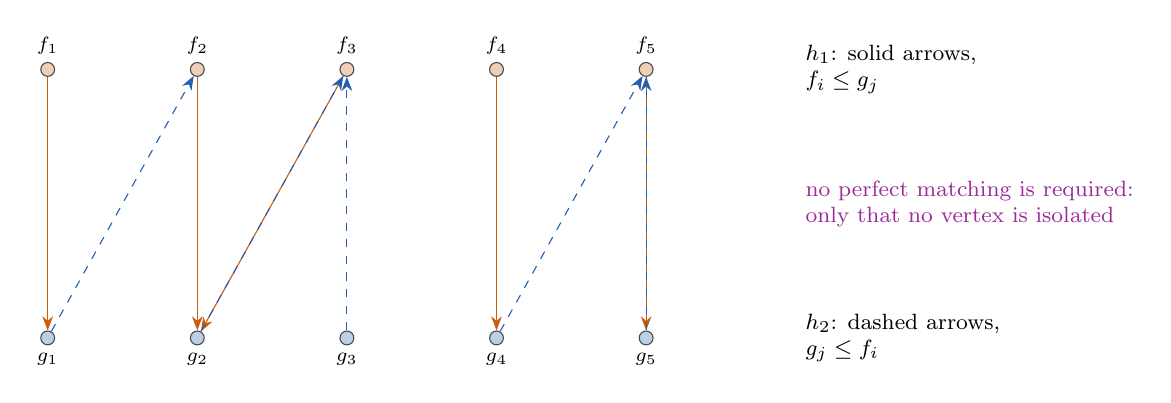
\begin{tikzpicture}[x=1.9cm,y=1.55cm,font=\footnotesize]
  \foreach \i in {1,...,5}{\node[latticept,fill=tagstructural!30] (f\i) at (\i,1.4) {};
    \node[font=\scriptsize,above=2pt] at (f\i) {$f_\i$};}
  \foreach \j in {1,...,5}{\node[latticept,fill=tagreducible!30] (g\j) at (\j,-0.8) {};
    \node[font=\scriptsize,below=2pt] at (g\j) {$g_\j$};}
  \foreach \i/\j in {1/1,2/2,3/2,4/4,5/5}{
    \draw[-{Stealth[length=1.8mm]},tagstructural] (f\i) -- (g\j);}
  \foreach \j/\i in {1/2,2/3,3/3,4/5,5/5}{
    \draw[-{Stealth[length=1.8mm]},tagreducible,dashed] (g\j) -- (f\i);}
  \node[anchor=west,align=left] at (6.0,1.4) {$h_1$: solid arrows,\\ $f_i \le g_{j}$};
  \node[anchor=west,align=left] at (6.0,-0.8) {$h_2$: dashed arrows,\\ $g_j \le f_{i}$};
  \node[anchor=west,align=left,text=bridgecol] at (6.0,0.3)
    {no perfect matching is required:\\ only that no vertex is isolated};
\end{tikzpicture}
\caption{Mutual cofinality.  The proof never chooses a canonical partner: it applies
\lean{iSup\_mono'} twice, which consumes exactly the existence of \emph{some}
out-neighbour.}
\end{figure}

\clearpage

\section{Arrow diagrams}

A complete lattice is a category with all (co)limits: objects are elements, there is one
arrow $a \to b$ exactly when $a \le b$, $\Sup$ is the colimit and $\Inf$ the limit.  Under
that dictionary each lemma of the development becomes a diagram, and each bridge of
\lean{RequestProject/Bridges.lean} becomes a functor.

\subsection{The proofs as commuting triangles}

Both collapse lemmas are a \lean{trans} of two equalities, i.e.\ a commuting triangle
whose slanted edge is the theorem.

\begin{figure}[ht]
\centering
\begin{minipage}{.48\textwidth}\centering
\begin{cdscale}{\textwidth}
\begin{tikzcd}[column sep=2.6cm,row sep=1.7cm]
\displaystyle\Sup_i \Sup_j F_{ij}
  \arrow[r,"\lab{iSup\_pprod}"]
  \arrow[dr,swap,pos=.42,"\lab{iSup₂\_eq\_iSup\_diagonal}"]
& \displaystyle\Sup_{p:\iota\times\iota} F_{p_1p_2}
  \arrow[d,"\lab{iSup\_eq\_iSup\_of\_cofinal}"] \\
& \displaystyle\Sup_k F_{kk}
\end{tikzcd}
\end{cdscale}
\\[4pt]{\footnotesize complete lattice: no side conditions}
\end{minipage}\hfill
\begin{minipage}{.48\textwidth}\centering
\begin{cdscale}{\textwidth}
\begin{tikzcd}[column sep=2.6cm,row sep=1.7cm]
\displaystyle\Sup_i \Sup_j F_{ij}
  \arrow[r,"\lab{ciSup\_pprod}"]
  \arrow[dr,swap,pos=.42,"\lab{ciSup₂\_eq\_ciSup\_diagonal}"]
& \displaystyle\Sup_{p:\iota\times\iota} F_{p_1p_2}
  \arrow[d,"\lab{ciSup\_eq\_ciSup\_of\_cofinal}"] \\
& \displaystyle\Sup_k F_{kk}
\end{tikzcd}
\end{cdscale}
\\[4pt]{\footnotesize conditionally complete: the horizontal arrow, and only it, consumes
\lean{bddAbove\_range\_uncurry}}
\end{minipage}
\caption{The same triangle twice.  Passing from the complete to the conditionally
complete world changes one edge label, not the shape.}
\end{figure}

\subsection{The binary-operation form as a zig-zag}

\lean{Golf.iSup\_op\_iSup\_diagonal} takes the two distributivity laws of the ambient
theory as parameters and produces the diagonal form; the proof is a three-step chain.

\begin{figure}[ht]
\centering
\begin{tikzcd}[column sep=2.4cm,row sep=1.4cm]
\mathrm{op}\bigl(\Sup_i f_i\bigr)\bigl(\Sup_j g_j\bigr)
  \arrow[r,"h_\ell"]
& \displaystyle\Sup_i \mathrm{op}\,(f_i)\bigl(\Sup_j g_j\bigr)
  \arrow[d,"\Sup_i h_r"] \\
\displaystyle\Sup_k \mathrm{op}\,(f_k)(g_k)
& \displaystyle\Sup_i\Sup_j \mathrm{op}\,(f_i)(g_j)
  \arrow[l,swap,"\lab{iSup₂\_eq\_iSup\_diagonal}"]
\end{tikzcd}
\caption{Instantiating $\mathrm{op}$ with \lean{(·+·)} and the pair
\lean{ENNReal.iSup\_add}/\lean{ENNReal.add\_iSup} gives \lean{ennreal\_iSup\_add\_iSup};
with \lean{(·*·)} and \lean{ENNReal.iSup\_mul}/\lean{ENNReal.mul\_iSup} the multiplicative
analogue --- same proof, new inputs.}
\end{figure}

\subsection{Currying and Fubini for colimits}

\lean{Golf.iSup\_pprod} is the lattice shadow of the Fubini theorem for colimits: the
colimit over a product category is the iterated colimit.

\begin{figure}[ht]
\centering
\begin{tikzcd}[column sep=1.8cm,row sep=1.3cm]
\iota\times\iota
  \arrow[r,"F"]
  \arrow[d,swap,"\mathrm{pr}_1"]
& \alpha \\
\iota
  \arrow[ur,swap,"{\Sup_j F(-,j)}"]
&
\end{tikzcd}
\qquad\qquad
\begin{tikzcd}[column sep=1.6cm,row sep=1.3cm]
\iota
  \arrow[r,"\Delta"]
  \arrow[dr,swap,"F\circ\Delta"]
& \iota\times\iota
  \arrow[d,"F"] \\
& \alpha
\end{tikzcd}
\caption{Left: the left Kan extension along $\mathrm{pr}_1$ is the row-supremum, and its
colimit is $\Sup_i\Sup_j F_{ij}$.  Right: the diagonal functor
$\Delta = $ \lean{CategoryTheory.Functor.diag}, whose composite with $F$ is the diagonal
family.  The theorem says the two colimits agree.}
\end{figure}

\subsection{The categorical bridge: the collapse \emph{is} finality of $\Delta$}

For a bimonotone family over a directed (= filtered) index, no order-theoretic argument
is needed at all: $\Delta$ is a final functor, and finality is precisely invariance of
colimits: this is
\lean{iSup\_prod\_eq\_iSup\_diagonal\_functor} in \lean{Bridges.lean}.

\begin{figure}[ht]
\centering
\begin{tikzcd}[column sep=2.1cm,row sep=1.35cm]
\iota
  \arrow[r,"\Delta"]
  \arrow[dr,swap,"F\Delta"]
& \iota\times\iota
  \arrow[d,"F"]
  \arrow[r,"\mathrm{colim}"]
& \operatorname{colim} F
  \arrow[d,equals,"\lab{Functor.Final.colimitIso}"{xshift=2mm}] \\
& \alpha
  \arrow[r,swap,"\mathrm{colim}"]
& \operatorname{colim} (F\Delta)
\end{tikzcd}
\qquad
\raisebox{1.1cm}{$\begin{aligned}
\operatorname{colim} F &= \Sup_{p}F_p &&\lab{colimit\_eq\_iSup}\\
\operatorname{colim} F\Delta &= \Sup_k F_{kk} &&\lab{colimit\_eq\_iSup}\\
\Delta \text{ final} &\ \Leftarrow\ \iota \text{ filtered}
  &&\lab{final\_diag\_of\_isFiltered}
\end{aligned}$}
\caption{The categorical route.  Directedness of $\iota$ enters as filteredness of the
index category; cofinality of the diagonal \emph{set} becomes finality of the diagonal
\emph{functor}.}
\end{figure}

\subsection{Transport along the bridges}

Each bridge of \lean{Bridges.lean} is a map of contexts.  What differs between them is
how much of the statement crosses: an order isomorphism carries hypothesis
\emph{and} conclusion, a sup-homomorphism only the conclusion, and duality carries
everything for free because it is the identity on propositions.

\begin{figure}[ht]
\centering
\begin{minipage}{.32\textwidth}\centering
\begin{tikzcd}[column sep=1.1cm,row sep=.95cm]
\alpha \arrow[r,"e","\sim"'] \arrow[d,swap,"\Sup"] & \beta \arrow[d,"\Sup"] \\
\alpha \arrow[r,swap,"e"] & \beta
\end{tikzcd}\\[3pt]
{\footnotesize\lean{OrderIso}: \\ \lean{e.map\_iSup}, both ways}
\end{minipage}\hfill
\begin{minipage}{.32\textwidth}\centering
\begin{tikzcd}[column sep=1.1cm,row sep=.95cm]
\alpha \arrow[r,"e"] \arrow[d,swap,"\Sup"] & \beta \arrow[d,"\Sup"] \\
\alpha \arrow[r,swap,"e"] & \beta
\end{tikzcd}\\[3pt]
{\footnotesize\lean{sSupHom}: \emph{not} injective; \\ only the conclusion crosses}
\end{minipage}\hfill
\begin{minipage}{.32\textwidth}\centering
\begin{tikzcd}[column sep=1.25cm,row sep=.95cm]
\alpha
  \arrow[r,bend left=25,"l"]
  \arrow[r,phantom,"\scriptstyle\bot"]
  \arrow[d,swap,"\Sup"]
& \beta
  \arrow[l,bend left=25,"u"]
  \arrow[d,"\Sup"] \\
\alpha \arrow[r,swap,"l"] & \beta
\end{tikzcd}\\[3pt]
{\footnotesize\lean{GaloisConnection}: the left \\ adjoint preserves $\Sup$}
\end{minipage}
\caption{Three functorial bridges of increasing weakness.  In all three the square
commutes, which is all the proof of the transported collapse uses
(\lean{simp only [← map\_iSup, iSup₂\_eq\_iSup\_diagonal]}).}
\end{figure}

\begin{figure}[ht]
\centering
\begin{tikzcd}[column sep=2.4cm,row sep=1.2cm]
\alpha
  \arrow[r,"{(-)^{\mathrm{od}}}","\sim"']
  \arrow[d,swap,"{\Sup_i\Sup_j F_{ij} = \Sup_k F_{kk}}"]
& \alpha^{\mathrm{od}}
  \arrow[d,"{\Inf_i\Inf_j F_{ij} = \Inf_k F_{kk}}"] \\
\mathrm{Prop}
  \arrow[r,equals,"\lab{Iff.rfl}"]
& \mathrm{Prop}
\end{tikzcd}
\caption{The duality bridge (\lean{Golf.Bridge.iSup₂\_diagonal\_iff\_dual}).  The
$\Inf$-statement in $\alpha^{\mathrm{od}}$ and the $\Sup$-statement in $\alpha$ are not
merely equivalent: they are the \emph{same} proposition, which is why every dual lemma
in \lean{Diagonal.lean} is proved by its primal with the single annotation
\lean{(α := αᵒᵈ)}.}
\end{figure}

\subsection{The bridge hub}

\begin{figure}[ht]
\centering
\begin{tikzpicture}[x=1cm,y=1cm,font=\footnotesize]
  \node[rounded corners=4pt,draw=diagcol,fill=diagcol!8,line width=1pt,
        align=center,inner sep=6pt] (T) at (0,0)
    {\textbf{diagonal collapse}\\[2pt]$\Sup_i\Sup_j F_{ij} = \Sup_k F_{kk}$};
  \tikzset{ctx/.style={rounded corners=3pt,draw=black!45,fill=white,align=center,
    inner sep=3.5pt,font=\scriptsize}}
  \node[ctx] (dual)  at (-5.2, 2.6) {$\alpha^{\mathrm{od}}$\\ duality};
  \node[ctx] (sets)  at (-5.6, 0.0) {$\mathrm{Set}\,\alpha$\\ \lean{IsCofinalFor}};
  \node[ctx] (lin)   at (-5.2,-2.6) {cond.\ complete\\ \emph{linear} order};
  \node[ctx] (iso)   at ( 0.0, 3.0) {$e : \alpha \simeq_o \beta$\\ order iso};
  \node[ctx] (hom)   at ( 5.3, 2.6) {$e : \mathrm{sSupHom}$\\ non-faithful};
  \node[ctx] (gal)   at ( 5.7, 0.0) {$l \dashv u$\\ Galois};
  \node[ctx] (cat)   at ( 5.2,-2.6) {$\mathrm{colim}$, $\Delta$ final\\ category theory};
  \node[ctx] (app)   at ( 0.0,-3.0)
    {$\enn$, $\mathbb{N}_\infty$, $\mathrm{Cardinal}$\\ applications};
  \foreach \n/\lab in {dual/{\lean{Iff.rfl}},sets/{\lean{sSup∘range}},
      lin/{no \lean{BddAbove}},iso/{hyp.\ \& concl.},hom/{concl.\ only},
      gal/{\lean{gc.l\_iSup}},cat/{finality},app/{instances}}{
    \draw[-{Stealth[length=2mm]},draw=bridgecol!80,line width=.7pt]
      (T) -- node[sloped,above,font=\tiny,text=bridgecol]{\lab} (\n);}
\end{tikzpicture}
\caption{One theorem, eight contexts.  The label on each arrow records how much of the
statement survives the transport --- the whole point of the bridge methodology is that
the cheapest context is not always the one the statement was posed in.}
\end{figure}

\clearpage

\section{The space of proofs of one lemma}

\lean{RequestProject/Variations.lean} proves each result of the development several
times, moving along the axes named in the proof-writing guides.  Those axes span a
Boolean lattice, so the catalogue of variants is literally a set of vertices of a cube ---
and one can see at a glance which corners are occupied.

\begin{figure}[ht]
\centering
\resizebox{\textwidth}{!}{%
\begin{tikzpicture}[x=1cm,y=1cm,font=\scriptsize]
  \tikzset{v/.style={circle,draw=black!65,fill=white,inner sep=1.6pt},
           occ/.style={v,fill=tagglue!45,draw=tagglue},
           emp/.style={v,fill=white,draw=black!35,densely dotted}}
  \def\dx{7.0}\def\dy{4.4}\def\dz{3.0}
  \coordinate (o000) at (0,0);
  \coordinate (o100) at (\dx,0);
  \coordinate (o010) at (0,\dy);
  \coordinate (o110) at (\dx,\dy);
  \coordinate (o001) at (\dz,{.62*\dz});
  \coordinate (o101) at ({\dx+\dz},{.62*\dz});
  \coordinate (o011) at (\dz,{\dy+.62*\dz});
  \coordinate (o111) at ({\dx+\dz},{\dy+.62*\dz});
  \foreach \a/\b in {o000/o100,o000/o010,o100/o110,o010/o110,
                     o001/o101,o001/o011,o101/o111,o011/o111,
                     o000/o001,o100/o101,o010/o011,o110/o111}
    {\draw[black!45] (\a) -- (\b);}
  \node[occ] at (o000) {}; \node[occ] at (o100) {};
  \node[occ] at (o010) {}; \node[occ] at (o110) {};
  \node[occ] at (o001) {}; \node[occ] at (o101) {};
  \node[emp] at (o011) {}; \node[occ] at (o111) {};
  \node[anchor=north east,align=right] at ($(o000)+(-.15,-.15)$)
    {\textbf{term, manual, one-liner}\\ \lean{cofinal\_v₁}, \lean{diagonal\_v₂}};
  \node[anchor=north west,align=left] at ($(o100)+(.15,-.15)$)
    {\textbf{tactic, manual, one-liner}\\ \lean{cofinal\_v₆} (\lean{<;>}),
     \lean{diagonal\_v₃}};
  \node[anchor=south east,align=right] at ($(o010)+(-.15,.15)$)
    {\textbf{term, manual, expanded}\\ \lean{cofinal\_v₂}};
  \node[anchor=south east,align=right] at ($(o110)+(-.15,.2)$)
    {\textbf{tactic, manual, expanded}\\ \lean{cofinal\_v₃},
     \lean{cofinal\_v₅} (\lean{calc})};
  \node[anchor=east,align=right,text=tagstructural] (labA) at (-0.5,2.6)
    {\textbf{term, automated}\\ \lean{ennreal\_mul\_pointfree},\\
     \lean{ennreal\_mul\_swap} (\lean{Function.swap})};
  \draw[thin,tagstructural!60] (labA.east) -- (o001);
  \node[anchor=west,align=left,text=tagstructural] at ($(o101)+(.25,-.1)$)
    {\textbf{tactic, automated, one-liner}\\ \lean{cofinal\_v₄} (\lean{simp only}),\\
     \lean{diagonal\_v₄} (\lean{rw}), \lean{grw}};
  \node[anchor=south east,align=right,text=black!45] at ($(o011)+(-.25,.25)$)
    {\emph{unoccupied}: automated\\ \emph{and} verbose in term mode};
  \node[anchor=west,align=left] at ($(o111)+(.25,.15)$)
    {\textbf{tactic, automated, expanded}\\ \lean{cardinal\_v₃} (\lean{simpa using})};
  % axes legend
  \begin{scope}[shift={(-1.2,-3.4)}]
    \draw[-{Stealth[length=2mm]},black!60] (0,0) -- ++(1.4,0)
      node[right,font=\scriptsize] {style: term $\to$ tactic};
    \draw[-{Stealth[length=2mm]},black!60] (0,0) -- ++(0,1.0)
      node[above,font=\scriptsize] {granularity};
    \draw[-{Stealth[length=2mm]},black!60] (0,0) -- ++(.85,.53)
      node[right,font=\scriptsize,xshift=1pt] {automation};
  \end{scope}
\end{tikzpicture}}
\caption{The design space of the mutual-cofinality lemma as the Boolean lattice
$B_3$.  Green vertices are realised by compiled proofs in \lean{Variations.lean}.}
\end{figure}

\subsection{A fourth axis: duality}

Duality is not a point of the cube but an involution acting on the whole of it: applying
$(-)^{\mathrm{od}}$ to any proof yields a proof of the $\Inf$-statement, and Lean accepts
it with a single type ascription.

\begin{figure}[ht]
\centering
\begin{tikzpicture}[x=1cm,y=1cm,font=\scriptsize]
  \draw[rounded corners=8pt,fill=tagglue!7,draw=tagglue!50] (-4.1,-1.4) rectangle (0.1,1.4);
  \draw[rounded corners=8pt,fill=tagreducible!7,draw=tagreducible!50]
    (4.1,-1.4) rectangle (8.3,1.4);
  \node[align=center] at (-2.0,.75) {$\Sup$-world\\ \lean{iSup₂\_eq\_iSup\_diagonal}};
  \node[align=center] at (-2.0,-.55) {\lean{iSup\_op\_iSup\_diagonal}\\
    \lean{ciSup₂\_eq\_ciSup\_diagonal}};
  \node[align=center] at (6.2,.75) {$\Inf$-world\\ \lean{iInf₂\_eq\_iInf\_diagonal}};
  \node[align=center] at (6.2,-.55) {\lean{iInf\_op\_iInf\_diagonal}\\
    \lean{ciInf₂\_eq\_ciInf\_diagonal}};
  \draw[{Stealth[length=2.4mm]}-{Stealth[length=2.4mm]},bridgecol,line width=1pt]
    (0.35,0) -- (3.85,0);
  \node[above=2pt,text=bridgecol,font=\scriptsize] at (2.1,0) {\lean{(α := αᵒᵈ)}};
  \node[below=2pt,text=bridgecol,font=\scriptsize] at (2.1,0) {cost: 0 lines};
\end{tikzpicture}
\caption{The dual half of \lean{Diagonal.lean} is generated, not written.}
\end{figure}

\subsection{From the abstraction to the applications}

\begin{figure}[ht]
\centering
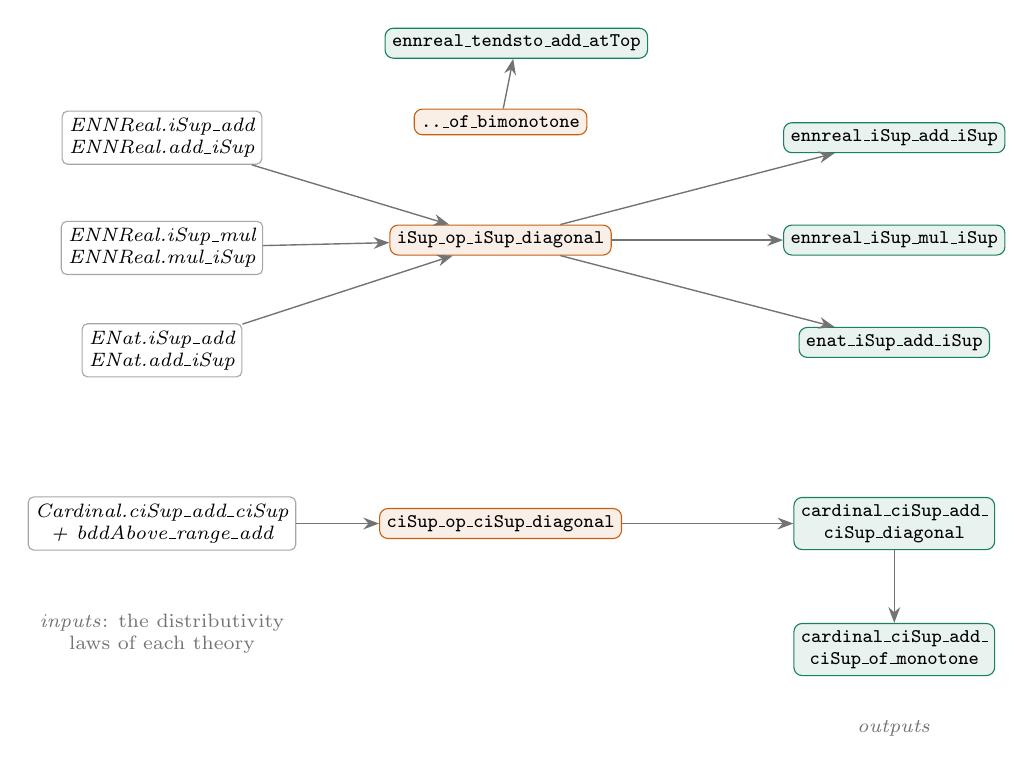
\begin{tikzpicture}[x=1cm,y=1cm,font=\scriptsize,
  every node/.style={inner sep=2.5pt}]
  \tikzset{core/.style={rounded corners=3pt,draw=tagstructural,fill=tagstructural!10,
      font=\ttfamily\scriptsize,align=center},
    appl/.style={rounded corners=3pt,draw=tagglue,fill=tagglue!10,
      font=\ttfamily\scriptsize,align=center},
    inp/.style={draw=black!35,fill=white,font=\scriptsize\itshape,align=center,
      rounded corners=2pt}}
  \node[core] (op)  at (0,2.0) {iSup\_op\_iSup\_diagonal};
  \node[core] (cop) at (0,-1.6) {ciSup\_op\_ciSup\_diagonal};
  \node[inp] (d1) at (-4.3,3.3) {ENNReal.iSup\_add\\ ENNReal.add\_iSup};
  \node[inp] (d2) at (-4.3,1.9) {ENNReal.iSup\_mul\\ ENNReal.mul\_iSup};
  \node[inp] (d3) at (-4.3,0.6) {ENat.iSup\_add\\ ENat.add\_iSup};
  \node[inp] (d4) at (-4.3,-1.6) {Cardinal.ciSup\_add\_ciSup\\ + bddAbove\_range\_add};
  \node[appl] (a1) at (5.0,3.3) {ennreal\_iSup\_add\_iSup};
  \node[appl] (a2) at (5.0,2.0) {ennreal\_iSup\_mul\_iSup};
  \node[appl] (a3) at (5.0,0.7) {enat\_iSup\_add\_iSup};
  \node[appl] (a4) at (5.0,-1.6) {cardinal\_ciSup\_add\_\\ciSup\_diagonal};
  \node[appl] (a5) at (5.0,-3.2) {cardinal\_ciSup\_add\_\\ciSup\_of\_monotone};
  \node[appl] (a6) at (0.2,4.5) {ennreal\_tendsto\_add\_atTop};
  \node[core] (bim) at (0,3.5) {..\_of\_bimonotone};
  \foreach \s in {d1,d2,d3}{\draw[use] (\s) -- (op);}
  \draw[use] (d4) -- (cop);
  \foreach \t in {a1,a2,a3}{\draw[use] (op) -- (\t);}
  \draw[use] (cop) -- (a4);
  \draw[use] (a4) -- (a5);
  \draw[use] (bim) -- (a6);
  \node[font=\scriptsize,text=black!55,align=center] at (-4.3,-3.0)
    {\emph{inputs}: the distributivity\\ laws of each theory};
  \node[font=\scriptsize,text=black!55] at (5.0,-4.2) {\emph{outputs}};
\end{tikzpicture}
\caption{The operation-level packaging turns each application into ``supply the two
distributivity lemmas''.  The multiplicative statement for $\enn$ and the additive one
for $\mathbb{N}_\infty$ cost two lines each, once the abstraction exists.}
\end{figure}

\subsection{Inventory}

\begin{center}\footnotesize
\begin{tabular}{@{}llr@{}}
\toprule
Statement & Axes exercised & Variants \\
\midrule
mutual cofinality & term/tactic, forward/backward, \lean{calc}, \lean{<;>} & 7 \\
diagonal corollary & corollary, standalone, \lean{rw}, duality & 6 \\
binary-operation form & \lean{trans} chain, \lean{simp\_rw}, point-free & 4 \\
boundedness helpers & set-level vs.\ family-level & 5 \\
conditionally complete collapse & currying-first vs.\ \lean{le\_antisymm}-first & 5 \\
\lean{Cardinal} payoff & \lean{rw}, \lean{simpa using}, linear-order bridge & 5 \\
$\enn$ & operation-level, categorical, \lean{sSupHom} transport & 6 \\
structural atoms & term/tactic, manual/automated & 6 \\
\bottomrule
\end{tabular}
\end{center}

\clearpage


\end{document}
